%\documentclass[11pt,a4paper]{report}

\documentclass{beamer}

\mode<presentation> {

% The Beamer class comes with a number of default slide themes
% which change the colors and layouts of slides. Below this is a list
% of all the themes, uncomment each in turn to see what they look like.

%\usetheme{default}
%\usetheme{AnnArbor}
%\usetheme{Antibes}
%\usetheme{Bergen}
%\usetheme{Berkeley}
%\usetheme{Berlin}
%\usetheme{Boadilla}
%\usetheme{CambridgeUS}
%\usetheme{Copenhagen}
%\usetheme{Darmstadt}
%\usetheme{Dresden}
%\usetheme{Frankfurt}
%\usetheme{Goettingen}
%\usetheme{Hannover}
%\usetheme{Ilmenau}
%\usetheme{JuanLesPins}
%\usetheme{Luebeck}
\usetheme{Madrid}
%\usetheme{Malmoe}
%\usetheme{Marburg}
%\usetheme{Montpellier}
%\usetheme{PaloAlto}
%\usetheme{Pittsburgh}
%\usetheme{Rochester}
%\usetheme{Singapore}
%\usetheme{Szeged}
%\usetheme{Warsaw}


% As well as themes, the Beamer class has a number of color themes
% for any slide theme. Uncomment each of these in turn to see how it
% changes the colors of your current slide theme.

%\usecolortheme{albatross}
%\usecolortheme{beaver}
%\usecolortheme{beetle}
%\usecolortheme{crane}
%\usecolortheme{dolphin}
%\usecolortheme{dove}
%\usecolortheme{fly}
%\usecolortheme{lily}
%\usecolortheme{orchid}
%\usecolortheme{rose}
%\usecolortheme{seagull}
%\usecolortheme{seahorse}
%\usecolortheme{whale}
%\usecolortheme{wolverine}

%\setbeamertemplate{footline} % To remove the footer line in all slides uncomment this line
%\setbeamertemplate{footline}[page number] % To replace the footer line in all slides with a simple slide count uncomment this line

%\setbeamertemplate{navigation symbols}{} % To remove the navigation symbols from the bottom of all slides uncomment this line
}

\usepackage[utf8]{inputenc}
\usepackage{graphicx}

\graphicspath{ {images/} }

\usepackage{amsmath,amsthm,amssymb,latexsym,amsfonts}



\usepackage{hyperref}
\usepackage{graphicx} % Allows including images
\usepackage{booktabs} % Allows the use of \toprule, \midrule and \bottomrule in tables



\title{(No) expresabilidad en primer orden}


\author{Guillermo Mosse} % Your name
\institute[UBA] % Your institution as it will appear on the bottom of every slide, may be shorthand to save space
{
Universidad de Buenos Aires\\ % Your institution for the title page
\medskip
\textit{billy.mosse@gmail.com} \\ % Your email address

}
\date{\today} % Date, can be changed to a custom date



\begin{document}


\begin{frame}
\titlepage % Print the title page as the first slide
\end{frame}


\begin{frame}
\frametitle{Enunciado}


%Definición: Dado un lenguaje de primer orden $\mathcal{L}$, decimos que una propiedad es expresable en primer orden si existe una fórmula $\phi$ tal que \\ para toda $\mathcal{L}$-estructura $\mathcal{A}$,  $\mathcal{A}$ $|$= $\phi$ sii $\mathcal{A} \in K$, donde $K$ es la clase de modelos que cumplen dicha propiedad.


\bigskip

%Ejercicio: una función $f$ se dice casi inyectiva si \\ \{$(x,y)$ $|$ $x \neq y \land f(x) = f(y)$\} es finito. Decidir si, dado $\mathcal{L}$ un lenguaje de primer orden con igualdad y un símbolo de función unario $f$, es expresable en primer orden la propiedad "$f$ es una función casi inyectiva".

Pr 7 ej 7: Sea $\mathcal{L}$ un lenguaje de primer orden con igualdad.

\bigskip
	a. Dar un conjunto de fórmulas $\Gamma$ tal que si $\Gamma$ es satisfacible para un modelo $\mathcal{M}$ (y una valuación $v$) entonces el dominio de $\mathcal{M}$ es infinito. Sugerencia: para cada $n$, escribir una fórmula $\phi_n$ que fuerce a que el modelo tenga al menos n elementos. 
	
	\bigskip
	b. Usando compacidad y el ítem anterior, demostrar que no existe ninguna fórmula $\phi$ tal que $\phi$ es satisfacible sii el dominio del modelo es finito.

\end{frame}


\begin{frame}
\frametitle{Resolución}

 a. Asumamos que para cada $n$ tenemos una fórmula $\phi_n$ que cumple lo dicho por la sugerencia.
 
 \pause
 
 \bigskip
 
 	Sea $\Gamma = \{\phi_n : n \in \mathbb{N}\}$. \textbf{Supongamos que el conjunto es satisfacible}. Entonces existe un modelo $\mathcal{M}$ (y una valuación $v$) tal que $\mathcal{M}\ |$= $\ \Gamma[v]$. Luego, para cada $n$, el dominio de
 	 $\mathcal{M}$ tiene más de $n$ elementos. Luego, ¡\textbf{es infinito}!
 	 
	
\end{frame}


\begin{frame}
\frametitle{Resolución}

Solo falta construir las $\phi_n$.

\pause

\bigskip


Para ellos introduzcamos todosDistintos$(x_1,\cdots,x_n)  \equiv x_1 \neq x_2\ \land$\\$ \land\  x_1 \neq x_3 \land \cdots x_1 \neq x_n \land x_2 \neq x_3 \land \cdots x_{n-1} \neq x_n$


todosDistintos NO es un predicado. Es un abuso de notación (parecido a las macros en computabilidad).Recordar que los predicados vienen dados con el lenguaje, así como las funciones y las constantes.

\pause

\bigskip

$\phi_n \equiv (\exists x_1,\cdots, x_n) todosDistintos(x_1,\cdots, x_n)$.

\bigskip

Si $\phi_n$ es satisfacible en un modelo $\mathcal{M}$ con dominio $\mathcal{A}$ y valuación $v$, por definición de las fórmulas, existen $a_1,\cdots, a_n \in \mathcal{A}$ tal que todos los elementos son distintos entre sí.

Se puede ver que también vale la vuelta, así que en realidad obtuvimos un si y solo si.
	
\end{frame}

\begin{frame}
\frametitle{b. Pasos de la demostración}

b. Supongamos que existe una fórmula $\phi$ tal que $\phi$ es satisfacible sii el dominio de $\mathcal{M}$ (el modelo) es finito.

Queremos llegar a un absurdo.

\pause

\bigskip 
Sea $\Gamma' = \Gamma \cup \{\phi\}$. Vamos a hacer lo siguiente:



\begin{enumerate}
		\item[1-] Probar que $\Gamma'$ es insatisfacible (probando que el modelo tendría que tener dominio finito e infinito a la vez)
		\item[2-] Probar que $\Gamma'$ es satisfacible (usando Compacidad)
		\item[3-] Por 1 y 2, llegar a un absurdo al suponer que existe una fórmula $\phi$ tal que $\phi$ es satisfacible sii el dominio de $\mathcal{M}$ es finito.
		\item[4-] Concluir que  no puede existir una $\phi$ así.		
	
\end{enumerate}
\end{frame}


\begin{frame}
\frametitle{$\Gamma'$ es \textbf{in}satisfacible}

Veamos que $\Gamma'$ es insatisfacible.

¿Qué significa que sea satisfacible? Pues que exista un modelo $\mathcal{M}$ con dominio $\mathcal{A}$ (y una valuación $v$) tal que $\mathcal{M}\ |$=$\ \Gamma'[v]$. \textbf{Supongamos que eso sucede}. Entonces, en particular, $\mathcal{M}\ |$=$\ \phi[v]$. Luego, por como es $\phi$, $\mathcal{M}$ tiene dominio finito.

\pause

\bigskip

Sin embargo, $\Gamma \subset \Gamma'$. Así que $\mathcal{M}\ |$=$\ \Gamma[v]$, así que, por el punto $a$, ¡$\mathcal{M}$ tiene dominio infinito!

\textbf{¡¡Absurdo!!} Así que $\Gamma'$ es insatisfacible. (O $\nexists\ \phi$, pero en ese caso ya ganamos)

\end{frame}


\begin{frame}
\frametitle{$\Gamma'$ es satisfacible}

Veamos ahora que $\Gamma'$ es satisfacible.
Por compacidad, basta ver que cualquier subconjunto finito es satisfacible.

\pause

\bigskip


Sea $\Gamma_{0} \subset \Gamma'$ un subconjunto finito, y
		$M = max (\{n: \phi_n \in \Gamma_0\}\cup \{1\})$.
		
		\pause 
		
		\bigskip
		
		Para el modelo que debemos construir, basta dar su dominio. Si elegimos $\mathcal{A} = \{1, \cdots, M\}$, como el dominio tiene $M$ elementos y el índice más grande de las $\phi_n$ que aparecen en $\Gamma_0$	es $M$, podemos afirmar, por el punto $a$, que $\forall\ \phi_n \in \Gamma_0$, $\phi_n$ es satisfacible. Además, si $\phi \in \Gamma_0$, $\phi$ es satisfacible porque el dominio del modelo es finito. Luego, $\Gamma_0$ es satisfacible.
		
				\pause \bigskip

		
		Entonces, por compacidad, como cada subconjunto finito es satisfacible, $\Gamma'$ es satisfacible.
		
\end{frame}

\begin{frame}
\frametitle{Conclusión}

Luego $\Gamma'$ es satisfacible, e insatisfacible. ¡¡Absurdo!! Luego no existe $\phi$ tal que $\phi$ es satisfacible sii el dominio de $\mathcal{M}$ es finito. $\square$


\end{frame}



\begin{frame}
\frametitle{Tarea}
Con una idea parecida, pueden hacer los ejercicios 8, 9 y 10 de la práctica 7, y el ejercicio 3 del recuperatorio de Lógica del 2015.
\end{frame}

\begin{frame}
\frametitle{Bibliografía}

Teóricas de LyC
\begin{itemize}
	\item Introducción a la lógica de primer orden: diapositivas 182 a 201
	\item Slide 236: enunciado del Teorema de Compacidad
	\item Slide 179: demostración del Teorema de Compacidad (para Lógica Proposicional)
	
\end{itemize}

\end{frame}


\begin{frame}
\frametitle{Fin}

\huge{¿Preguntas?} \bigskip


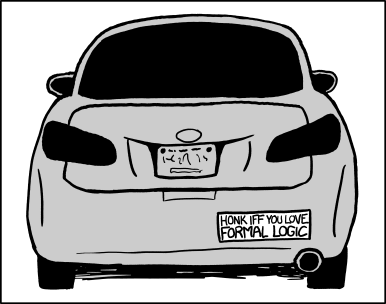
\includegraphics[scale=0.5]{formal_logic.png}
\\
\small{Note that this implies you should NOT honk solely because I stopped for a pedestrian and you're behind me.}

\end{frame}

%El ¡Recordemos! lo hago en el pizarrón. Qué recuerdo?
%Qué es una valuación, que está definida sobre las variables proposicionales y %que se extiende a las otras cosas,
%y que lo de arriba es que para toda valuación sea válida.


%
%\begin{frame}
%
%\begin{itemize}
%\item Hola \alt<1>{bla}{ble}
%\item Hola \alt<2>{bla}{ble}
%
%\end{itemize}
%
%\end{frame}



%Ejercicio (tarea): Sea L un lenguaje de primer orden con igualdad y un símbolo de predicado binario R. Decidir si es posible expresar en primer orden la propiedad que afirma que existe k $\in$ N tal que todo elemento se relaciona a lo sumo con k elementos distintos.


\end{document}

%
%\tableofcontents
%\part{Addition and Subtraction}
%\chapter{Addition} \chaptercontent
%\chapter{Subtraction} \chaptercontent
%\part{Multiplication and Division}
%\chapter{Multiplication} \chaptercontent
%\chapter{Division} \chaptercontent
%\end{document}